\documentclass[tikz,border=8pt]{standalone}
% Shared look for every TikZ diagram. Load with \input{../../tools/tikz-style.tex}
\usepackage[sfdefault]{roboto}
\usetikzlibrary{arrows.meta, positioning, shapes.geometric, calc, fit, backgrounds}
\definecolor{cblue}{HTML}{4C78A8}
\definecolor{corange}{HTML}{F58518}
\definecolor{cgreen}{HTML}{54A24B}
\definecolor{cred}{HTML}{E45756}
\definecolor{cpurple}{HTML}{B279A2}
\definecolor{cgrey}{HTML}{6B6B6B}
\tikzset{
  every picture/.style={font=\sffamily, line width=1.2pt},
  box/.style={draw=#1, fill=#1!12, rounded corners=4pt, align=center, inner sep=7pt, minimum height=1.1cm},
  box/.default=cgrey,
  arrow/.style={-{Stealth[length=3mm]}, draw=cgrey, line width=1.4pt},
  title/.style={font=\sffamily\bfseries\Large},
  note/.style={font=\sffamily\small, text=cgrey, align=center},
}
\AtBeginDocument{\hyphenpenalty=10000 \exhyphenpenalty=10000}

% One free node of the room's harmonic potential and its four neighbours, 0.05 m apart (pf.harmonic_solve, rounded to
% 4 places): the node at (3.5, 3.6) holds 0.9374, the average of 0.9429, 0.9336, 0.9482 and 0.9247 (3.7494 / 4 =
% 0.93735). The lowest neighbour, 0.9247, is the one above, towards the door: the next step of the robot.
\begin{document}
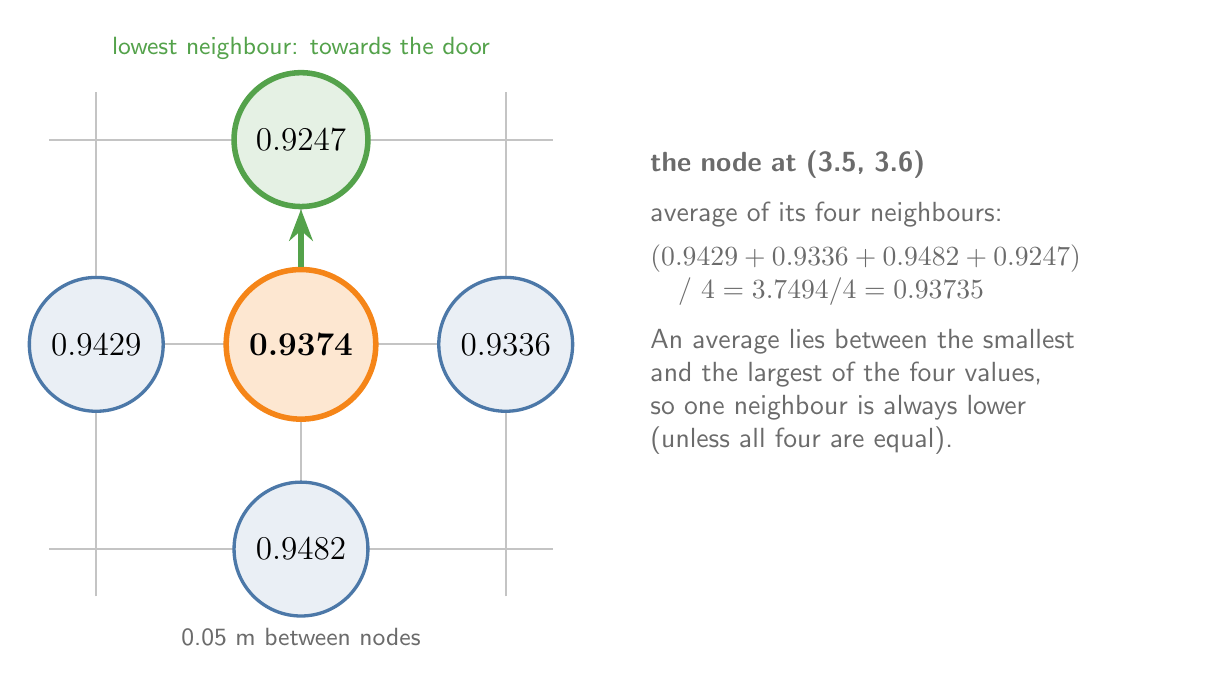
\begin{tikzpicture}[every node/.append style={font=\large}]
  \foreach \x in {-2.6,0,2.6} \draw[cgrey!40, line width=0.8pt] (\x,-3.2) -- (\x,3.2);
  \foreach \y in {-2.6,0,2.6} \draw[cgrey!40, line width=0.8pt] (-3.2,\y) -- (3.2,\y);
  \node[circle, draw=corange, fill=corange!20, minimum size=1.9cm, line width=2pt] (c) at (0,0) {\textbf{0.9374}};
  \node[circle, draw=cblue, fill=cblue!12, minimum size=1.7cm] (l) at (-2.6,0) {0.9429};
  \node[circle, draw=cblue, fill=cblue!12, minimum size=1.7cm] (r) at (2.6,0) {0.9336};
  \node[circle, draw=cblue, fill=cblue!12, minimum size=1.7cm] (d) at (0,-2.6) {0.9482};
  \node[circle, draw=cgreen, fill=cgreen!15, minimum size=1.7cm, line width=2pt] (u) at (0,2.6) {0.9247};
  \draw[-{Stealth[length=4mm]}, draw=cgreen, line width=2.2pt] (c) -- (u);
  \node[note, anchor=south, text=cgreen] at (u.north) {lowest neighbour: towards the door};
  \node[note, anchor=north] at (d.south) {0.05 m between nodes};
  \node[note, anchor=north west, align=left, text width=6.6cm, font=\sffamily\normalsize] at (4.3,2.6)
     {\textbf{the node at (3.5, 3.6)}\\[6pt]
      average of its four neighbours:\\[4pt]
      $(0.9429 + 0.9336 + 0.9482 + 0.9247)$\\
      $\quad /\ 4 = 3.7494 / 4 = 0.93735$\\[6pt]
      An average lies between the smallest\\ and the largest of the four values,\\
      so one neighbour is always lower\\ (unless all four are equal).};
\end{tikzpicture}
\end{document}
